\capitulo{5}{Aspectos relevantes del desarrollo del proyecto}

En este apartado voy a comentar, en forma de resumen temporal, las partes más importantes en el desarrollo del proyecto. Hablaré desde decisiones importantes de diseño hasta problemas que me han llevado mucho tiempo resolver. He considerado que lo mejor para este apartado es dividir los aspectos relevantes en secciones.

\section{Comienzo con APACE e investigación}
APACE Burgos presentó el proyecto AVC a los premios de Fundación Vodafone para buscar financiación y poder realizar el proyecto. Este premio se lo concedieron y fue entonces cuando se pusieron en contacto con la Universidad de Burgos para poder desarrollar el proyecto. Es en ese momento en el que me comunican la posibilidad de hacer este proyecto como Trabajo Fin de Grado.

Tuvimos una serie de reuniones con APACE donde nos expusieron el problema, que era la falta de herramientas de comunicación para personas con parálisis cerebral gravemente afectadas y su consiguiente exclusión tanto social como laboral. También discutimos sobre las posibles soluciones que tendría el problema hasta que llegamos a la solución conceptual que define el proyecto hoy en día, una aplicación intuitiva y accesible que nos permite interpretar sonidos de personas con parálisis cerebral.

En las primeras semanas empecé a estudiar como se hacía una aplicación Android, a la par que comenzaba la parte de investigación para ayudar a mi compañero en el proyecto, Sergio Chico Carrancio. Los artículos de investigación que estudié estaban relacionados con el problema al que nos enfrentábamos, extracción de características de audios y clasificación de sonidos. Entre los artículos que leí destacan el uso de distintos métodos de preprocesado del audio para, por ejemplo, eliminar los silencios, como se puede ver en el artículo sobre reconocimiento de sonidos de animales~\cite{yeo2011animal}. Después del preprocesado del audio se pasa a la extracción de características a partir de éste. Muchos de los métodos más usados para la extracción de características en audios usan la escala de \textit{Mel}, explicada en el apartado ~\ref{mel}. Y por último, tras obtener las características de los audios procesados, ya tenemos la entrada para nuestros métodos de clasificación. Es en éstos donde podemos ver más variación ya que podemos tener métodos sencillos como puede ser un \textit{KNN} o métodos más complejos como puede ser las Redes Neuronales~\cite{pandeya2018domestic}.

\section{Prototipo aplicación y estudio sobre el audio}
Como mi parte en este proyecto no era la investigación, sino el desarrollo de las aplicaciones y el servidor, dejé la parte de investigación para empezar a desarrollar la primera aplicación. En este primer prototipo me basé en un tutorial que enseñaba como usar \textit{MediaRecorder}, una clase que he utilizado hasta el final para grabar audios con los dispositivos \textit{Android}.

La finalidad de esta primera aplicación, cuya pantalla inicial se ven en la figura ~\ref{fig:prototipo}, en un principio era para realizar la recogida de datos necesarios para la investigación de la que se ocupaba el investigador Sergio Chico. En esta aplicación las personas encargadas de grabar los audios eran los que tenían que apuntar a mano y enviarnos a través de correo el conjunto de datos, es decir, el audio junto a ciertas opciones adicionales que luego se comentan en el siguiente apartado. Pero tras varias reuniones con APACE se llegó a la conclusión de que iba a ser muy costoso para las personas encargadas (familiares y cuidadores) generar datos y apuntar a mano, así que se planteó  una segunda aplicación para la recogida de datos, pasando esta primera aplicación a ser una aplicación prototipo. 

Cabe destacar dentro de esta aplicación dos funcionalidades que añadí. La primera es la generación automática del nombre que tiene el fichero de audio de la salida, y la segunda funcionalidad es la petición de permisos de acceso al almacenamiento del dispositivo y de grabación de audios. Esta funcionalidad y el código que la implementa se ha usado en las 3 aplicaciones del proyecto y me costó mucho tiempo conseguir que funcionasen, ya que la ejecución de la aplicación se paraba y cerraba por no tener los permisos concedidos. Esto lo solucioné gracias a añadir los permisos en el \textit{AndroidManifest.xml} y a la siguiente función que pide los permisos.

\begin{lstlisting}[language={Java}]
private void askForPermissions() {
	String[] perm = {Manifest.permission.RECORD_AUDIO,Manifest.permission.WRITE_EXTERNAL_STORAGE};
	
	if(ContextCompat.checkSelfPermission(this.getApplicationContext(),perm[0]) != PackageManager.PERMISSION_GRANTED || ContextCompat.checkSelfPermission(this.getApplicationContext(),perm[1]) != PackageManager.PERMISSION_GRANTED){
		requestPermissions(perm,1234);
	}
}	
\end{lstlisting}

\begin{figure}
	\centering
	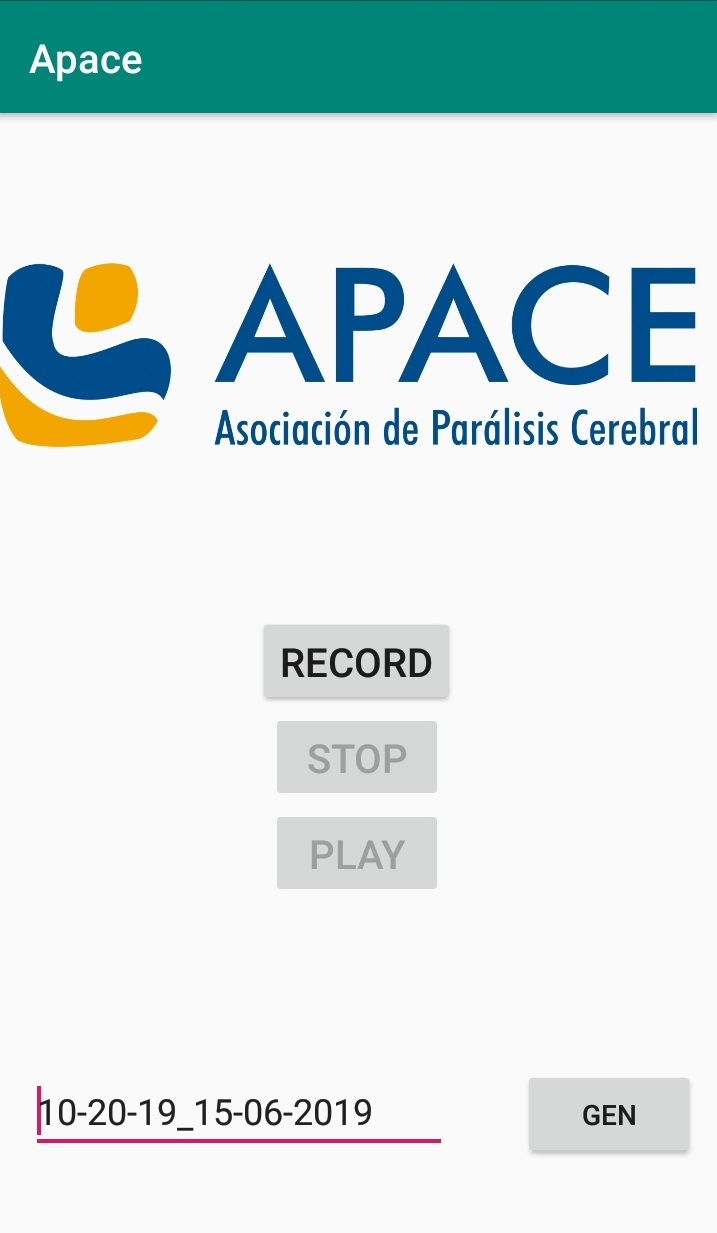
\includegraphics[scale=0.3]{prototipo}
	\caption{Aplicación prototipo.}
	\label{fig:prototipo}
\end{figure}

A la vez que desarrollaba el prototipo estaba investigando acerca de qué formato y qué códec de audio iba mejor para la configuración del \textit{MediaRecorder} y es aquí donde realizamos el estudio del audio. Aquí nos encontramos con el problema de que en \textit{Android} y en concreto con \textit{MediaRecorder} no podíamos codificar, es decir, grabar en cualquier formato. Por ejemplo, vimos que \textit{mp3} con \textit{MediaRecorder} en \textit{Android} solo permite decodificar. Tras realizar el estudio para encontrar el mejor formato, no conseguimos obtener un formato que tuviese un códec sin pérdida, así que intentamos obtener el formato con la mayor calidad posible. Es por ello que elegimos el códec \textit{AAC-LC}, formato \textit{mp4}, con un \textit{bitrate} de 128kbps y un \textit{sampling rate} de 48kHz~\cite{mediarecorder}.

\section{Obtención de las opciones adicionales}
Al comienzo del proyecto se comentó con APACE que quizás los audios no serían suficientes para poder realizar una clasificación exacta de las emociones, pero la clasificación de una respuesta binaria si que se tomaba posible de clasificar solo con el audio. Es por ello que para este problema nos planteamos el uso de unas opciones adicionales que pudiesen dar más información al clasificador.

APACE nos mandó una primera versión de estas opciones adicionales, que se obtuvieron pasando un formulario a las familias de la asociación y a profesionales en la materia. En estas primeras opciones adicionales teníamos un conjunto de opciones por cada una de las emociones que queríamos clasificar, que se pueden ver en la imágenes~\ref{fig:opcdolor}, ~\ref{fig:opcenfado}, ~\ref{fig:opctristeza} y ~\ref{fig:opchambre}. En estas imágenes en la columna de la izquierda están las opciones iniciales, y en la columna derecha las opciones condensadas por APACE. Como se puede observar son demasiadas opciones, tantas que darían demasiadas dimensionalidades a los datos de entrada del clasificador, lo que haría muy complicado el entrenamiento y la clasificación posterior. Es por ello que decidimos tratar de resumir estas opciones, las cuales han sido las que han llegado al final del proyecto y se pueden ver en la tabla~\ref{tabla:opcfinal}.

\begin{figure}
	\centering
	
\includegraphics[width=\textwidth]{dolor}
	\caption{Opciones adicionales proporcionadas por APACE de la emoción dolor.}
	\label{fig:opcdolor}
\end{figure}

\begin{figure}
	\centering
	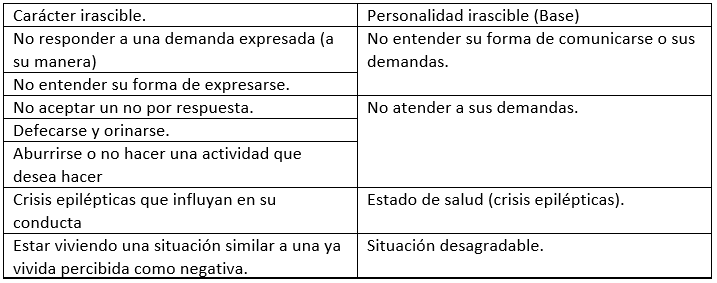
\includegraphics[width=\textwidth]{enfado}
	\caption{Opciones adicionales proporcionadas por APACE de la emoción enfado.}
	\label{fig:opcenfado}
\end{figure}

\begin{figure}
	\centering
	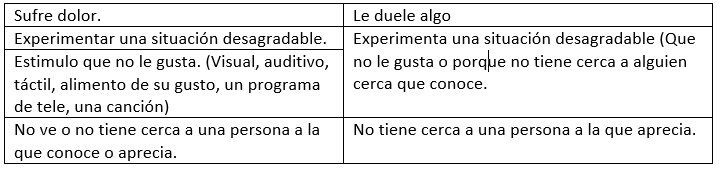
\includegraphics[width=\textwidth]{tristeza}
	\caption{Opciones adicionales proporcionadas por APACE de la emoción tristeza.}
	\label{fig:opctristeza}
\end{figure}

\begin{figure}
	\centering
	
\includegraphics[width=\textwidth]{hambre}
	\caption{Opciones adicionales proporcionadas por APACE de la emoción hambre.}
	\label{fig:opchambre}
\end{figure}

\tablaSmall{Opciones adicionales finales}{l c}{opcfinal}
{ \multicolumn{1}{l}{\textbf{Opción}} & \textbf{Posibles valores} \\}{ 
	Actualmente está enfermo & Sí/No\\
	Sufre dolor crónico & Sí/No\\
	Ha sido operado recientemente & Sí/No\\
	Ha dormido/descansado mal & Sí/No\\
	Ha estado/está en una mala postura & Sí/No\\
	El entorno que lo rodea no es agradable & Sí/No\\
	Las personas que lo rodean no son conocidas & Sí/No\\
	Ha comido & Antes/A su hora/Tarde\\
	Ha comido & Mucho/Normal/Poco/Nada\\
} 

\section{Desarrollo de la aplicación de recogida de datos}
Como ya he comentado, en una reunión con APACE nos transmitieron el cambio que querían hacer en la aplicación prototipo para la recogida de datos, el cual se  que la selección de las opciones adicionales y de la emoción o respuesta relacionada se pudiese hacer desde la aplicación. Con este cambio tuve que empezar a crear la segunda aplicación a partir de la aplicación prototipo. Desde APACE se nos comentó que esta aplicación debía ser lo más sencilla posible de usar, ya que algunas familias, que podían recoger datos, no tienen mucho dominio de las tecnologías. 

Esta aplicación fue bastante más complicada de hacer, ya que era la primera vez que iba a trabajar y tener en cuenta la navegabilidad entre pantallas de la aplicación. Además, la aplicación tenía que ser lo más lineal posible, por lo que primero me puse a diseñar una interfaz, la cual se puede ver en la figura~\ref{fig:interrd}.

Una vez diseñada la interfaz pasé a aprender a navegar por las pantallas de una aplicación \textit{Android} y a desarrollar la aplicación. Del desarrollo de esta aplicación cabe destacar:
\begin{itemize}
	\item Navegabilidad intuitiva gracias al uso de los \textit{ActivityResult}, que permiten terminar un \textit{Activity} con un resultado según ésta haya acabado de forma correcto o incorrecta. Esta funcionalidad la he usado para poder habilitar los botones, ya que se pidió que la aplicación fuese simple y lineal.
	\item En la pantalla de selección de la emoción o respuesta relacionada con los datos generados no se permite ni dejarla vacía, ni elegir una opción de la columna de emociones y otra de la columna respuesta, ni elegir las opciones sí y no de forma simultanea.
	\item Uso de ficheros \textit{csv} para la almacenar y enviar tanto las opciones adicionales como la emoción o respuesta asociado, usando la librería \textit{OpenCSV}~\cite{opencsv}.
	\item Persistencia y carga de los datos en todas las pantallas gracias a una creación de carpetas bien definidas y al uso de una estructura de datos bien definida. Esto nos permite volver a entrar a una de las pantallas y tener los datos que se habían generado. Ocurre tanto en la pantalla de grabación del audio, como en las pantallas de selección de opciones y de selección de emoción o respuesta.
	\item Generación de comprimidos con el archivo del audio y los archivos \textit{csv}, para poder enviarlos con mayor facilidad.
	\item Envío por correo del comprimido para poder recogerlo y estudiarlo. 
\end{itemize}

Este último punto hubo que discutirlo con los tutores, porque nuestras opciones para enviar el comprimido eran o hacerlo directamente con un servidor o usar un correo electrónico. Al final, decidimos usar el correo electrónico ya que no teníamos tiempo de desplegar un servidor y la aplicación tenía que estar en marcha lo antes posible para que se empezase a generar datos con los que el investigador colaborador, Sergio Chico, pudiese hacer el estudio.

Además, un problema habitual en el desarrollo de servidores en los trabajos fin de grado es que al finalizar estos los datos almacenados en ellos se pierden. Esto puede ser muy importante, ya que en años posteriores otro alumno puedo partir de ese Trabajo Fin de Grado, pero ya no tendría datos. Esta es una ventaja más del uso del correo, ya que por mucho que se desconecte el servidor, siempre se puede acceder a los datos almacenados en el correo, por lo que nunca se pierden.

La interfaz final de la aplicación se puede ver en la figura~\ref{fig:interfinalrd}.
\begin{figure}
	\centering
	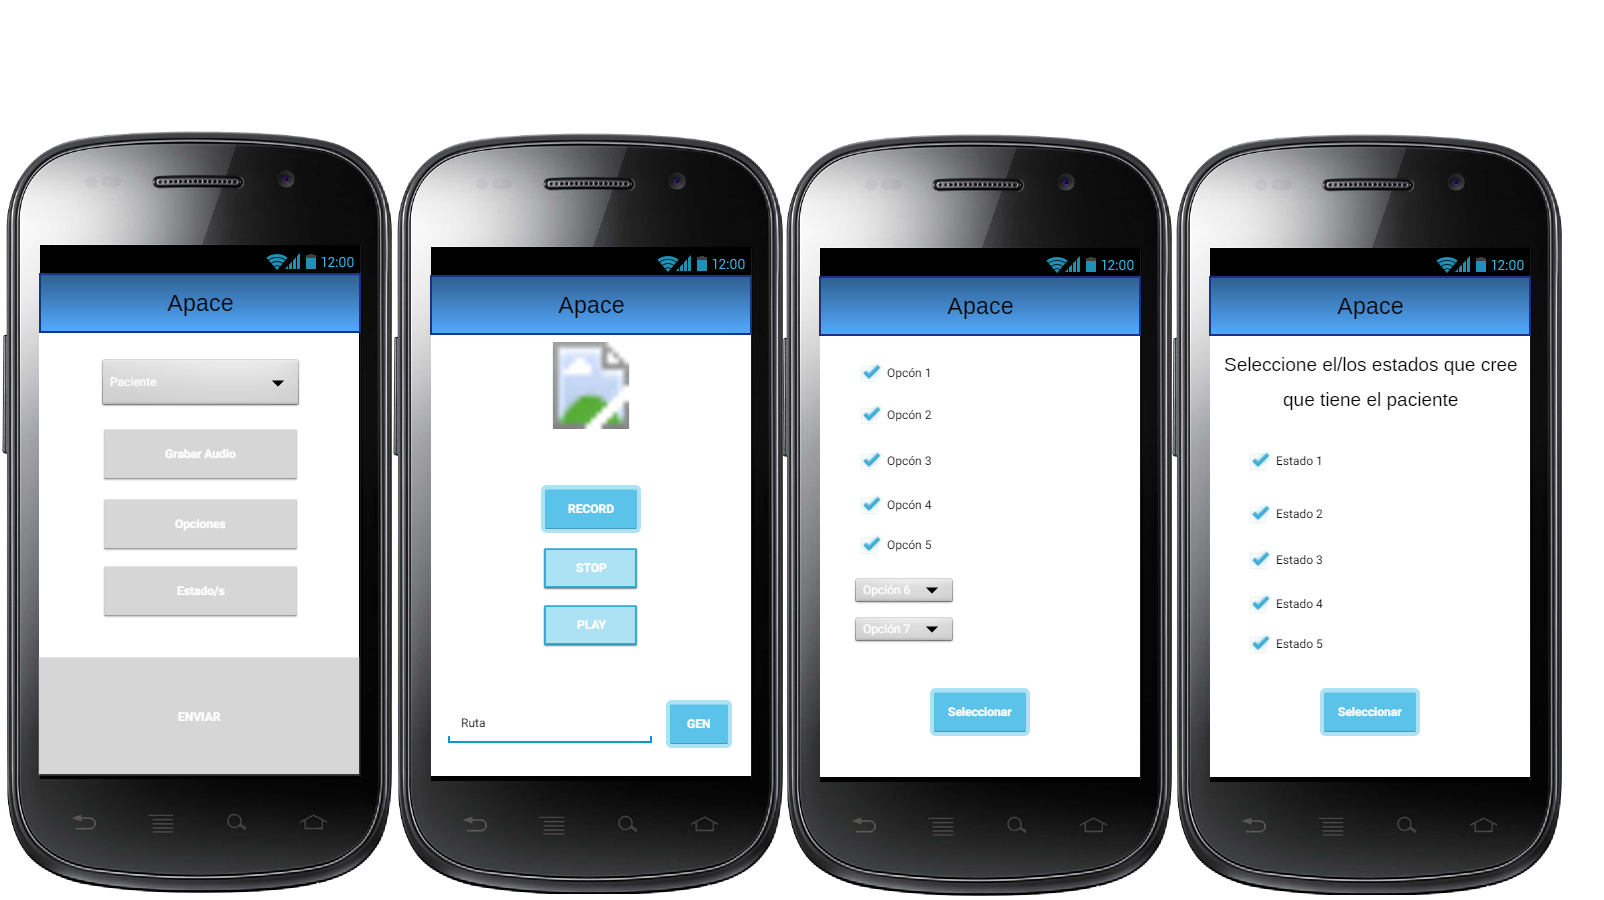
\includegraphics[width=\textwidth]{interfaz}
	\caption{Diseño interfaz aplicación recogida de datos.}
	\label{fig:interrd}
\end{figure}
\begin{figure}
	\centering
	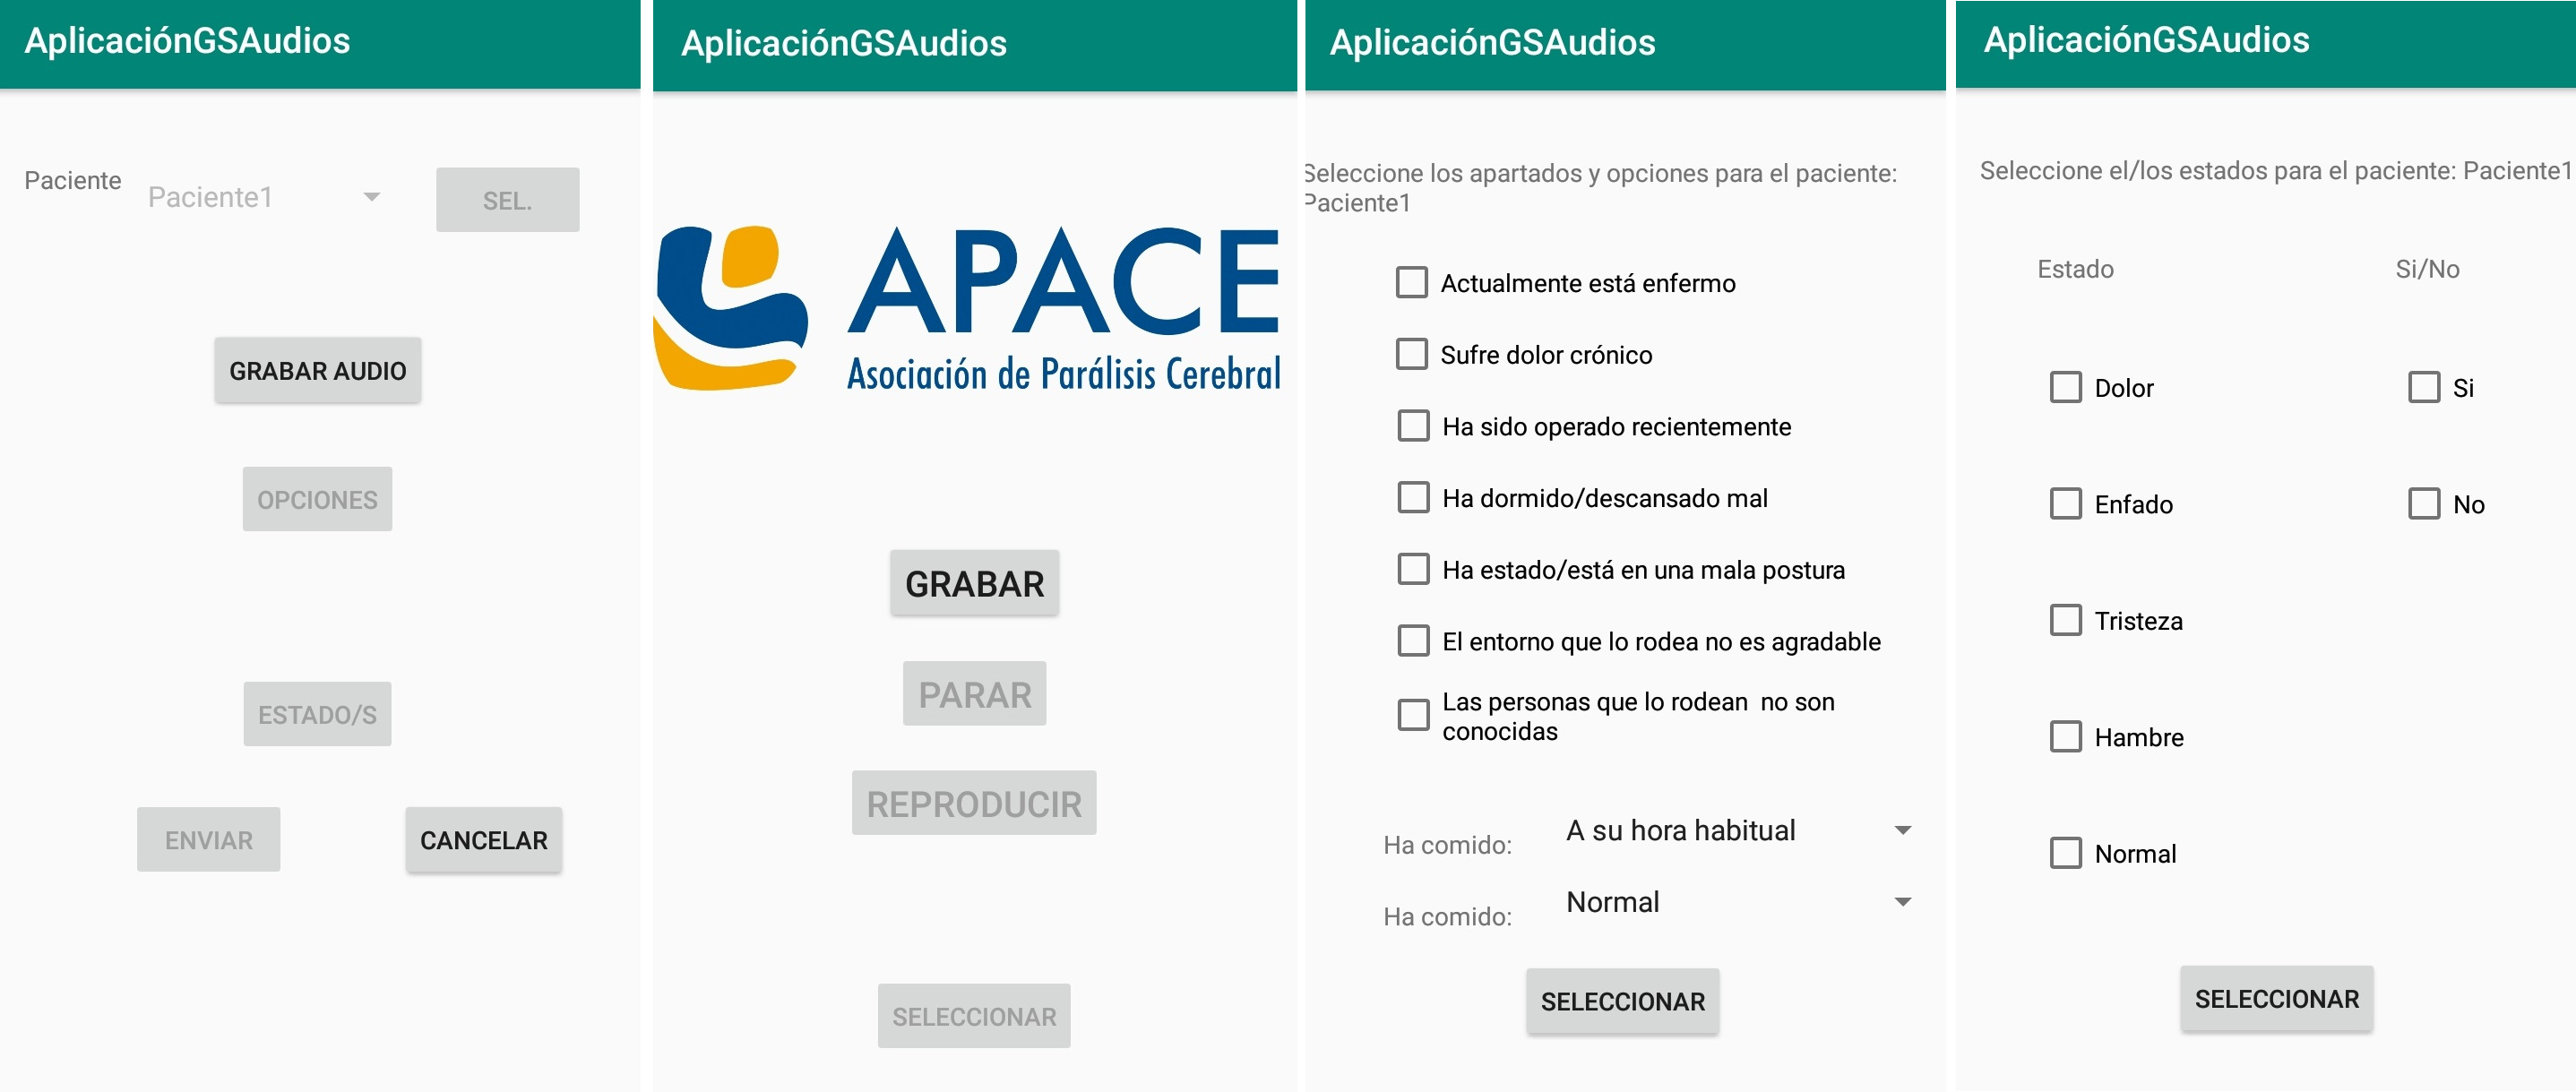
\includegraphics[width=\textwidth]{interfinalrd}
	\caption{Interfaz aplicación recogida de datos.}
	\label{fig:interfinalrd}
\end{figure}

\section{Obtención de sonidos prototipo}
Tras finalizar la aplicación para la generación de datos, y sus presentaciones en APACE que posteriormente comentaré, nos encontramos con un problema que ya veíamos venir desde prácticamente el comienzo del proyecto, la falta de datos. Obviamente no podíamos forzar a los pacientes a hacer sonidos, y menos cuando las emociones con las que nos pidió APACE trabajar son negativas (dolor, hambre, tristeza y enfado).

En una reunión comentamos las posibles opciones que teníamos, y éstas eran o esperar a que antes de la entrega tuviésemos suficientes datos como para al menos tener un clasificador para una persona, o intentar imitar los sonidos para poder generar algunos datos con los que el investigador colaborador, Sergio Chico, pudiese empezar a trabajar. Con el fin de poder tener una aplicación prototipo final que nos permitiese clasificar audios decidí generar de forma artificial los audios con los que entrenar al clasificador.

Esta probablemente sea una de las tareas que más me ha costado en todo el proyecto, ya que tenía que seguir unos pasos, para que los datos que generase tuviesen el mayor sentido posible. Estos pasos para cada una de las emociones y sí/no eran:
\begin{itemize}
	\item Descargar algunos ejemplos que ya hubiesen enviado, para tener algo en lo que basarme.
	\item Grabar un audio propio intentando ceñirme lo máximo posible a los audios descargados anteriormente.
	\item En las emociones, estudiar las opciones adicionales para saber cuales se suelen repetir más con una emoción.
	\item Grabar alrededor de unos 20 audios por cada emoción y sí/no, teniendo que escucharlos, valorar si son o no válidos y poner las opciones adicionales correspondientes para cada una de la grabaciones.
\end{itemize}
\section{Desarrollo de la aplicación de interpretación - AVC}
Una vez que ya contábamos con suficientes datos como para que el investigador colaborador, Sergio Chico, empezase a estudiar las mejores formas de extraer las características del audio y poder clasificarlo, yo empecé a desarrollar la aplicación final. Es la aplicación más importante en el proyecto, ya que es la que se más se usará y la que dará esa mejora en la vida de las personas con parálisis cerebral que buscamos.

Lo primero que realicé fue el diseño de la interfaz junto con un equipo especializado de APACE, el cual me facilitó el logotipo de la aplicación que se puede ver en la figura~\ref{fig:logo}. Diseñé al rededor de 6 interfaces iniciales, en las cuales se destaca el uso desde el principio de botones de información para dar mayor accesibilidad a la aplicación, y para las cuales este equipo me fue indicando cambios y mejoras hasta llegar al diseño final, que aparece en la figura~\ref{fig:dinteravc}. 

Cabe destacar un cambio muy importante que me comentaron desde APACE, y es que las opciones adicionales no se cumplimentasen cada vez que queremos hacer una interpretación, sino que estas se almacenasen en el servidor y solo se modificasen cuando sea necesario.

\begin{figure}
	\centering
	
\includegraphics[width=\textwidth]{LOGO}
	\caption{Logotipo de la aplicación.}
	\label{fig:logo}
\end{figure}

\begin{figure}
	\centering
	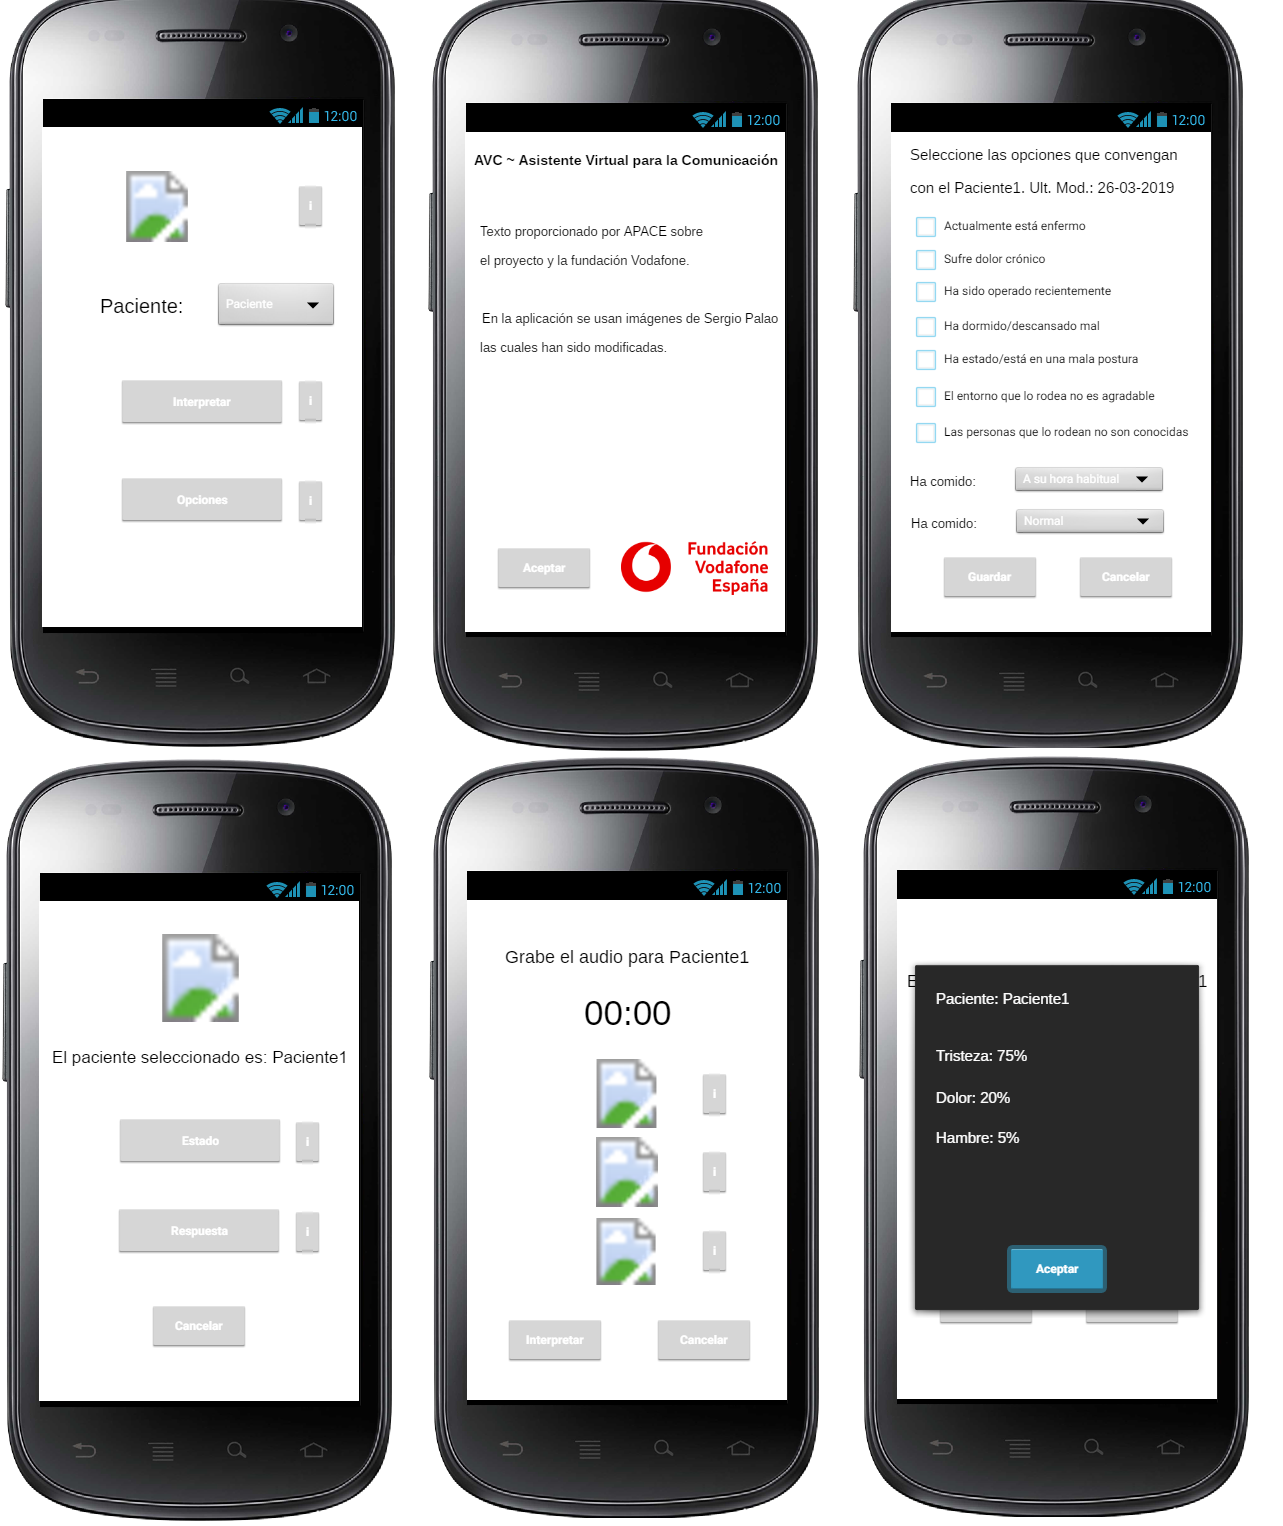
\includegraphics[width=\textwidth]{disintavc}
	\caption{Diseño interfaz aplicación AVC.}
	\label{fig:dinteravc}
\end{figure}

Esta es la aplicación más importante y compleja del proyecto. Es por ello que es a la que sin duda he dedicado más tiempo. En el desarrollo de esta primera versión sin conexión al servidor cabe destacar los siguientes apartados:
\begin{itemize}
	\item \textbf{Creación de una estructura de ficheros:} necesario para poder controlar los distintos ficheros con los que trabaja la aplicación, siendo la raíz de esta estructura donde se almacena el audio grabado. En la carpeta \textit{/config} tenemos el fichero \textit{csv} donde se almacena al paciente por defecto.
	\item \textbf{Comprobación y restauración de la estructura de ficheros}: para que al iniciarse la aplicación lo primero que se compruebe sea que la estructura de ficheros existe, y si falta alguna carpeta y/o fichero los genere.
	\item \textbf{Implementación de la selección del paciente por defecto:} que al abrir de nuevo la aplicación aparezca en el \textit{spinner} del paciente el último paciente seleccionado antes de cerrar la aplicación. Esto se ha conseguido gracias al conocimiento sobre el control de ficheros \textit{csv} obtenido en el desarrollo de la aplicación de generación de datos con \textit{OpenCSV}~\cite{opencsv}.
	\item \textbf{Continua implicación por parte de APACE:} necesaria para conseguir que la aplicación fuese lo más accesible posible. Esto dio como resultado algunos cambios en la interfaz, desde las primeras versiones que aparecen en la figura~\ref{fig:primver} donde me comentaron que los degradados no eran lo mejor para personas con alguna discapacidad visual, a una segunda versión donde, a parte de eliminar el degradado, se modificó el color al color que ellos me dijeron, que era el azul, teniendo así que modificar todas las imágenes para que los textos estuviesen en blanco~\ref{fig:segver}. Por último, eliminé todos los píxeles blancos de las imágenes a mano, porque al tener las imágenes con un fondo azul los píxeles blancos se ven mucho. Esto nos lleva a la última versión de la interfaz~\ref{fig:verfi}.
	\item \textbf{Uso de diálogos para mejorar la accesibilidad:} con \textit{AlerDialog} en los botones de información para mostrar información sobre el botón que está al lado. Estos diálogos están escritos en lectura fácil gracias a la Universidad de Salamanca. Además, al abrir el diálogo se reproduce por audio el texto escrito para dar una mayor accesibilidad~\ref{fig:dia}.
\end{itemize}
Como se puede observar, el desarrollo de esta aplicación ha sido orientado casi totalmente a conseguir una mayor accesibilidad. Este punto ha sido tan importante en el equipo de desarrollo porque desde un principio teníamos la idea de que hasta los compañeros de estas personas gravemente afectadas del centro de día de APACE pudiesen utilizarlo, para así poder entender a sus compañeros.

\begin{figure}
	\centering
	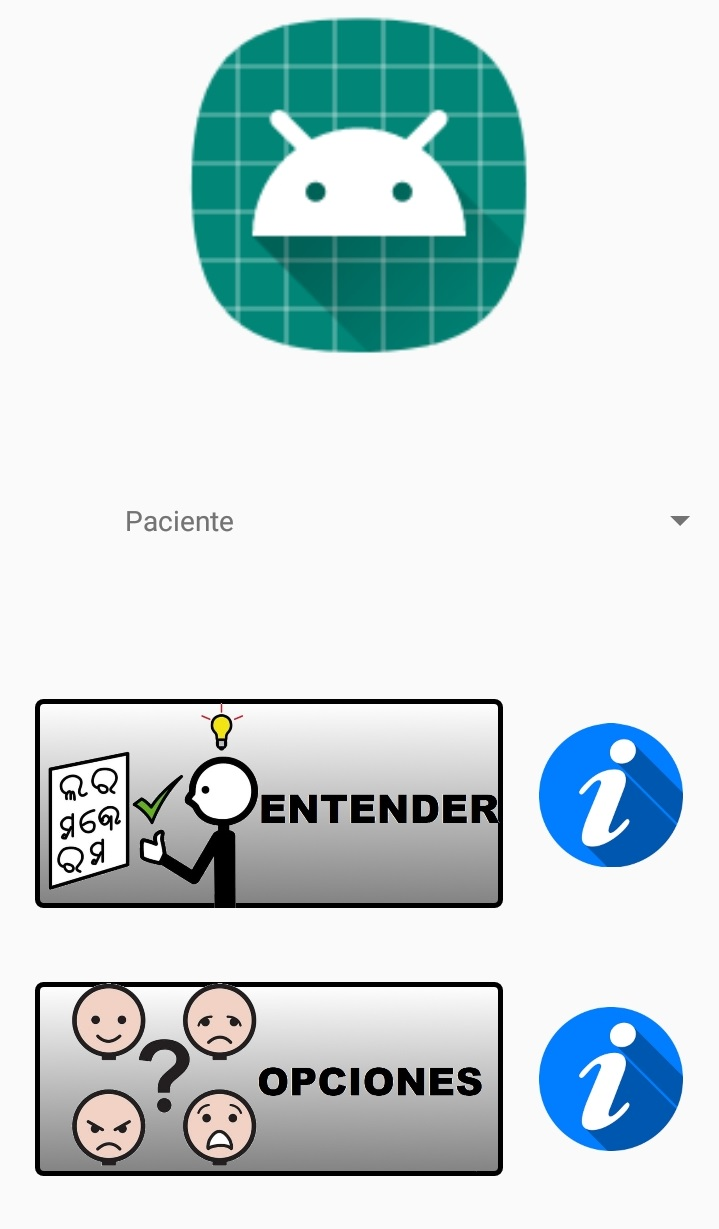
\includegraphics[scale=0.3]{primerasversiones}
	\caption{Primera versión de la interfaz.}
	\label{fig:primver}
\end{figure}
\begin{figure}
	\centering
	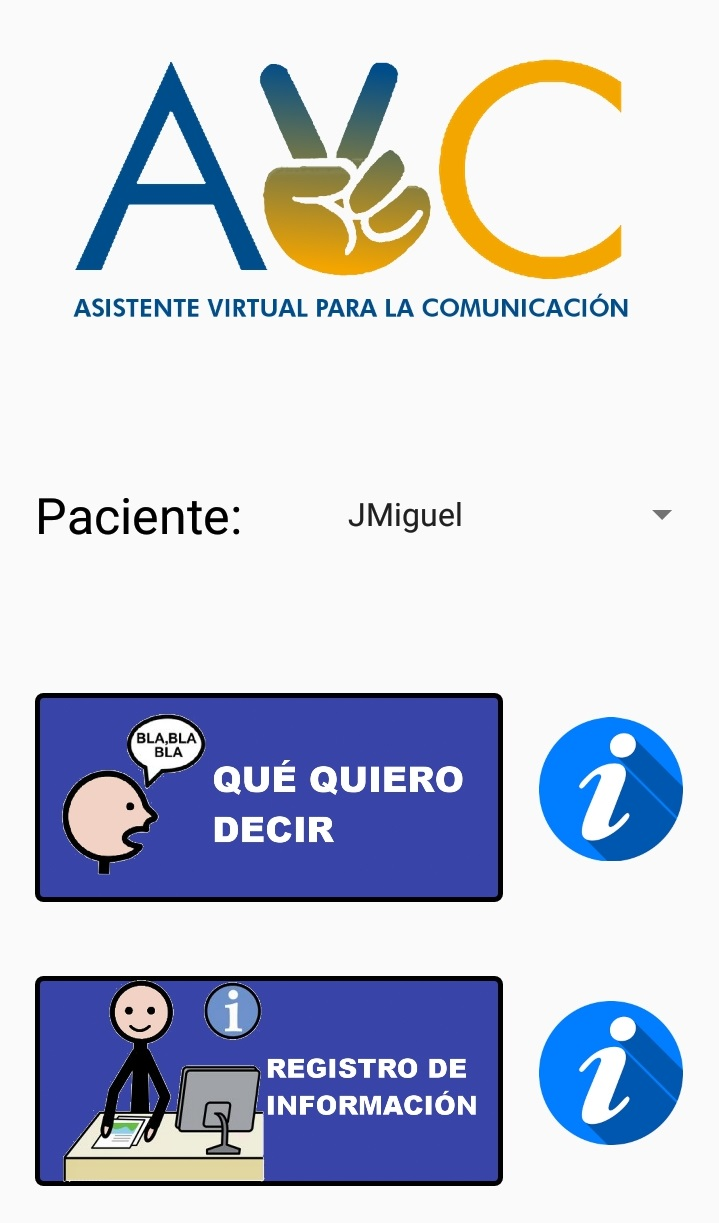
\includegraphics[scale=0.3]{segundaversion}
	\caption{Segunda versión de la interfaz.}
	\label{fig:segver}
\end{figure}
\begin{figure}
	\centering
	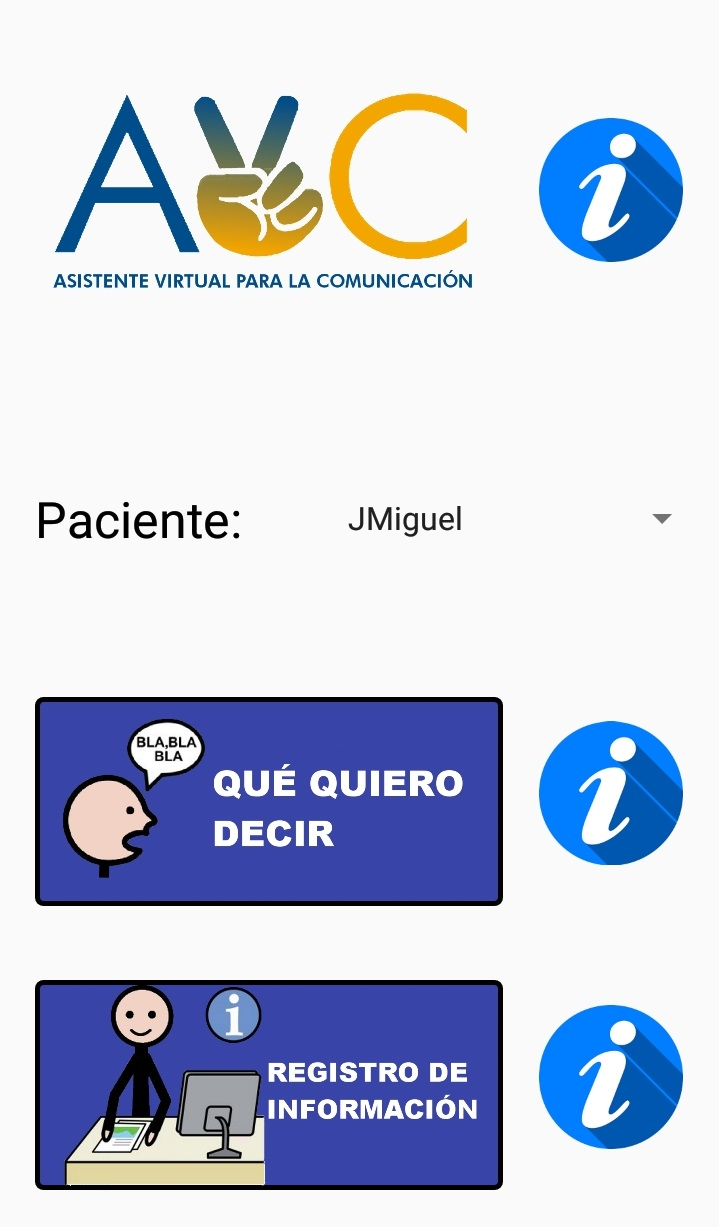
\includegraphics[scale=0.3]{versionfinal}
	\caption{Versión final de la interfaz, donde no se observan los bordes blancos en los pictogramas, como se puede ver en la segunda versión.}
	\label{fig:verfi}
\end{figure}
\begin{figure}
	\centering
	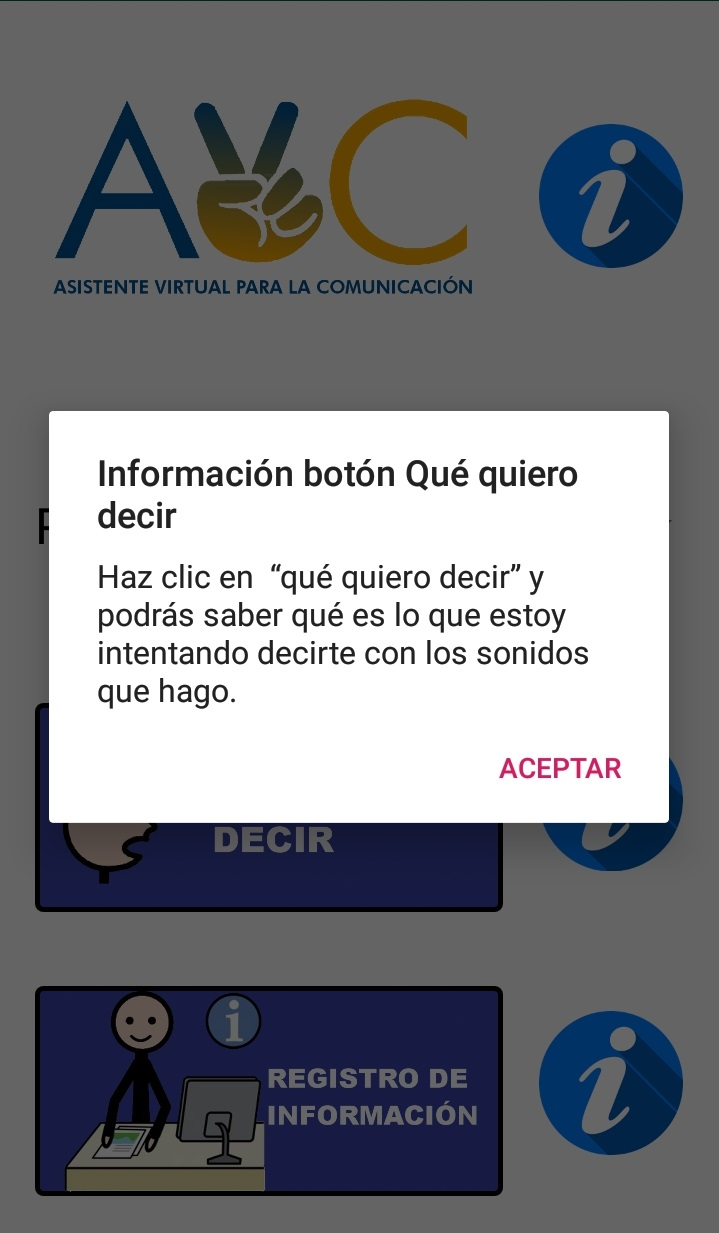
\includegraphics[scale=0.3]{dialogo}
	\caption{Ejemplo de diálogo en lectura fácil.}
	\label{fig:dia}
\end{figure}

Después de terminar el desarrollo de la aplicación empecé con la fase de test de ésta. En ella primero diseñé los test unitarios para probar la lógica y la creación de los distintos elementos de la aplicación y los implementé, y después, usando Espresso~\cite{espresso}, diseñé e implementé los test de integración para comprobar la correcta colaboración entre las distintas partes de la aplicación. Un ejemplo de este diseño de los test se puede ver en la figura~\ref{fig:ditestun}~\cite{vypcn,vypcb,vypti}.

\begin{figure}
	\centering
	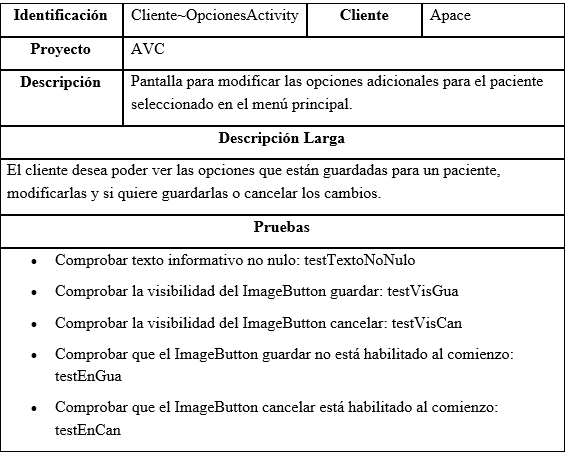
\includegraphics[width=\textwidth]{distest}
	\caption{Diseño de test unitarios de OpcionesActivity.}
	\label{fig:ditestun}
\end{figure}

Tras probar los distintos test descubrí unos cuantos \textit{bugs}, que es la función de los test. Hubo un \textit{bug} en particular que me llevó mucho tiempo resolver, el cual afectaba a cómo se generaba la estructura de datos, ya que hay algunos test que prueban esa funcionalidad eliminando partes o toda la estructura de ficheros de la aplicación.

Además, realicé un tipo especial de test llamado \textit{Monkey Test}~\cite{monkeytest}, que consiste en, a través de una prueba de estrés pulsando aleatoriamente puntos de la pantalla, probar la consistencia de la aplicación. Gracias a este test descubrí un error importante en la pantalla de grabación de audios, ya que la grabación no se paraba cuando se retrocedía a la pantalla anterior pulsando el botón \textit{back} del dispositivo.
\section{Desarrollo del servidor}
Tras tener una primera versión de la aplicación tocaba empezar a desarrollar el servidor. Para ello primero tenía que aprender a usar \textit{Flask}~\cite{flask}, ya que era la primera vez que iba a desarrollar un servidor.

El primer paso que tuve que dar fue el de elegir el tipo de \textit{request} con el cual quería hacer las peticiones al servidor. Elegí el tipo \textit{post} porque tenía más conocimiento acerca de este tipo de \textit{request HTTP} y por recomendación de compañeros~\cite{sdintro,sdhttp}.

El segundo paso fue el diseño de los distintos métodos del servidor. Tras el diseño se decidí usar 4 métodos \textit{post} en el servidor:
\begin{itemize}
	\item \textbf{Nombre:} API/Nombres, \textbf{caso de uso:} CU1, \textbf{descripción:} Devuelve la lista de usuarios de los que hay un método entrenado preparado para clasificar. Esta lista está en un fichero csv en el servidor, \textbf{parámetros:} Token, \textbf{salida:} JSON con una cadena con la lista de los nombres.
	\item \textbf{Nombre:} API/ObtOpciones, \textbf{caso de uso:} CU2, \textbf{descripción:} Devuelve los valores de las opciones adicionales del paciente seleccionado, leyendo el fichero csv del servidor indicado, \textbf{parámetros:} Paciente y token, \textbf{salida:} JSON con una cadena con la lista de las opciones almacenadas.
	\item \textbf{Nombre:} API/GuaOpciones, \textbf{caso de uso:} CU3, \textbf{descripción:} Almacena las opciones que se envían desde la aplicación para el paciente seleccionado, \textbf{parámetros:} Paciente, lista de valores y token, \textbf{salida:} Resultado booleano de la operación.
	\item \textbf{Nombre:} API/Clasifica, \textbf{caso de uso:} CU5 y CU6, \textbf{descripción:} Ejecuta el modelo entrenado para el paciente pasado con el audio pasado y con las opciones adicionales que están actualmente guardadas en el servidor., \textbf{parámetros:} Paciente, tipo de interpretación, audio y token, \textbf{salida:} JSON con una cadena con los datos sobre la emoción o respuesta y sus porcentajes.
\end{itemize}

Después, cree la estructura necesaria en el servidor, esta estructura es:

\dirtree{%
	.1 root.
	.2 Modelos.
	.2 Opciones.
	.2 Temp.
	.2 pacientes.csv.
	.2 apiserver.py.
	.2 clip.py.
}

En la carpeta \textit{Modelos} es donde se almacenan los distintos modelos ya entrenados. En la carpeta \textit{Opciones} se encuentran todos los \textit{csv} con las opciones adicionales guardadas para cada paciente. En \textit{Temp} tenemos los ficheros de audio temporales de cada interpretación, éstos se eliminarán después de devolver al cliente el resultado. El fichero \textit{pacientes.csv} tiene la lista de pacientes entrenados y los ficheros \textit{apiserver.py} y \textit{clip.py} son los ficheros encargados de la extracción de características y de la clasificación.

Por último, implementé todos los métodos en \textit{Python}, haciendo todas las respuestas con \textit{jsonify}~\cite{jsonify}. Algunos aspectos que se pueden destacar del desarrollo del servidor son:
\begin{itemize}
	\item \textbf{Control de concurrencia:} sobre todo en el método de clasificación donde el servidor recibe varios archivos de audios que tiene que saber identificar correctamente. Esto se ha conseguido gracias a la creación dinámica de nombres para los audios en el servidor.
	\item \textbf{Resultado aleatorio:} a parte de obviamente tener el clasificador para los datos que generé, quise añadir más usuarios en la aplicación para así poder modificar las opciones y comprobar el correcto funcionamiento, pero para ello también necesitaba un clasificador para estos audios. Es por ello que creé una función que genera resultados válidos aleatorios con los cuales responder a las interpretaciones de pacientes no entrenados.
\end{itemize}

Tras haber implementado cada uno de los métodos tenía que probarlo, pero como la aplicación final no estaba desarrollada, puesto que aun no estaban unidas ambas partes, aplicación y servidor, tuve que usar una herramienta para poder hacer \textit{request HTTP} desde el ordenador.

\section{Conexión de aplicación y servidor}
Una vez tuve la aplicación y el servidor desarrollados solo quedaba unir ambas partes. Para ello primero tuve que aprender a realizar \textit{post} en \textit{Android}. Decidí hacer los \textit{post} con paso de parámetros por \textit{url}, lo que después me llevó un problema con el audio que contaré posteriormente.

Al implementar los métodos \textit{post} me encontré con un problema. La conexión al servidor, que está desplegado en un portátil al cual tengo que acceder a través de una dirección IP. Eso cuando lo estaba implementando en casa era sencillo, ya que esta IP apenas cambiaba y solo hay un router en red, pero la presentación del proyecto se iba a hacer en sitios como la universidad, o el mismo APACE, donde nos encontramos con redes más complejas donde apuntar a un dispositivo no es tan fácil como poner la IP. Es por ello que decidí usar el programa \textit{noWifi} en el portátil en donde está desplegado el servidor, ya que me permite crear un red a la cual apuntar con los dispositivos \textit{Android} siempre con la dirección 192.168.137.1 y al puerto definido en \textit{Flask}, el puerto 5000.

Al implementar el cuarto método \textit{post} en \textit{Android}, el método que me permite enviar la petición de clasificación, me encontré con un gran problema. ¿Cómo conseguir pasar un archivo de audio en \textit{mp4} a un servidor a través de un método en el cual le paso los parámetros por texto en la \textit{url}? La respuesta la encontré en la codificación a \textit{Base64}, que me permite transformar mi archivo de audio en texto, el cual puedo pasar en la \textit{url} y luego decodificarlo en el servidor haciendo la operación inversa. 

Al desarrollar el paso a \textit{Base64} me encontré con otro problema, puesto que la codificación que usaba en \textit{Android} no se decodificaba bien en el servidor \textit{Python}. Me llevó mucho tiempo solventarlo, ya que intenté usar muchos métodos para codificar en \textit{Base64}, pero ninguno daba resultado porque todos los métodos que probaba al decodificarlo en el servidor me daba como resultado un fichero corrupto. Además, se juntó otro impedimento, y es que la librería de \textit{Base64} de \textit{Java} subía el API mínimo varias versiones, por lo que de usarlo no podríamos cumplir nuestro objetivo técnico de usar como máximo la API 23 de \textit{Android}~\cite{base64java}. Tras probar muchos métodos pasé directamente a imprimir el resultado de la codificación para ver si podía verse el problema, y en efecto, no se correspondía con la codificación esperada por el servidor. Fue entonces cuando cambié el fichero de audio para pasar a codificar un fichero de texto, encontré el método, \textit{Base64.encodeToString} que funcionaba correctamente en \textit{Android}, y luego lo probé con el fichero de audio y por fin funcionó.

\begin{lstlisting}[language={Java}]
String baudio=null;

try {
	byte[] b = new byte[(int) aufile.length()];
	FileInputStream fis = new FileInputStream(aufile);
	fis.read(b);
	baudio = Base64.encodeToString(b, Base64.NO_WRAP);
} catch (FileNotFoundException e) {
	e.printStackTrace();
} catch (IOException e) {
	e.printStackTrace();
}	
\end{lstlisting}

En el código se ve como se hace la codificación a \textit{Base64}. Es importante el uso del \textit{Base64.NO\_WRAP}, ya que lo que hace es codificarlo todo como una única cadena, debido a que otras configuraciones lo que hacen es introducir saltos de línea que impiden la correcta decodificación.

Por último, quise dar una mayor seguridad al servidor para que no se pueda acceder a una de las peticiones desde fuera de la aplicación. Esto lo conseguí añadiendo un \textit{token} de seguridad como parámetro a todos los métodos. Fue entonces cuando pensé que puede haber una serie de errores con el servidor que se podrían agrupar, codificar, describir y dar una solución. Es así como se me ocurrió hacer una estandarización de los errores de la aplicación en la conexión con el servidor. Estos tienen un código asociado, y con él una descripción de por qué ocurre y como solucionarlo, como se ve en la tabla~\ref{tabla:errores}. Un ejemplo de un mensaje de error se puede ver en la figura~\ref{fig:error}.
	
\begin{table}
	\resizebox{\textwidth}{!}{%
		\begin{tabular}{@{}llll@{}}
			\toprule
			Error & \textbf{Descripción}                                                                & \textbf{Causa}                                                                                                                                                                               & \textbf{Solución}                                                                                                                                    \\ \midrule
			Er1   & \begin{tabular}[c]{@{}l@{}}No se puede \\ acceder al servidor.\end{tabular}         & \begin{tabular}[c]{@{}l@{}}Este error se da cuando el servidor\\  está caído.\end{tabular}                                                                                                   & \begin{tabular}[c]{@{}l@{}}Avisar al Administrador para que \\ reinicie el servidor.\end{tabular}                                                    \\
			Er2   & \begin{tabular}[c]{@{}l@{}}Token de \\ seguridad\\  incorrecto.\end{tabular}        & \begin{tabular}[c]{@{}l@{}}O se ha corrompido la aplicación\\  cambiando el token de seguridad \\ o el token de seguridad ha cambiado\\  sin ser actualizado en su dispositivo.\end{tabular} & \begin{tabular}[c]{@{}l@{}}Avisar al Administrador para que \\ le pase de nuevo la aplicación.\end{tabular}                                          \\
			Er3   & \begin{tabular}[c]{@{}l@{}}Lista de nombres \\ vacía en el servidor.\end{tabular}   & \begin{tabular}[c]{@{}l@{}}La lista con los nombres en el\\  servidor está vacía.\end{tabular}                                                                                               & \begin{tabular}[c]{@{}l@{}}Avisar al Administrador para \\ que recupere el archivo.\end{tabular}                                                     \\
			Er4   & \begin{tabular}[c]{@{}l@{}}Lista de nombres \\ no encontrada.\end{tabular}          & \begin{tabular}[c]{@{}l@{}}El fichero con la lista de los \\ pacientes en el servidor no está.\end{tabular}                                                                                  & \begin{tabular}[c]{@{}l@{}}Avisar al Administrador para \\ que recupere el archivo.\end{tabular}                                                     \\
			Er5   & \begin{tabular}[c]{@{}l@{}}Opciones del \\ paciente no\\  encontradas.\end{tabular} & \begin{tabular}[c]{@{}l@{}}El fichero con las opciones \\ adicionales del paciente no \\ está en el servidor.\end{tabular}                                                                   & \begin{tabular}[c]{@{}l@{}}Avisar al Administrador para \\ que recupere el archivo.\end{tabular}                                                     \\
			Er6   & \begin{tabular}[c]{@{}l@{}}No hay \\ conexión \\ a Internet.\end{tabular}           & \begin{tabular}[c]{@{}l@{}}No tener conexión ni Wifi \\ ni Datos Móviles.\end{tabular}                                                                                                       & \begin{tabular}[c]{@{}l@{}}Conectarse a una red con acceso\\  a Internet.\end{tabular}                                                               \\
			Er7   & \begin{tabular}[c]{@{}l@{}}Fichero del \\ paciente vacío.\end{tabular}              & \begin{tabular}[c]{@{}l@{}}El fichero del paciente con las\\  opciones está vacío en el servidor.\end{tabular}                                                                               & \begin{tabular}[c]{@{}l@{}}Avisar al Administrador para \\ que recupere el archivo.\end{tabular}                                                     \\
			Er8   & \begin{tabular}[c]{@{}l@{}}Fichero de \\ clasificación \\ no existe.\end{tabular}   & \begin{tabular}[c]{@{}l@{}}No existe el fichero con el que se\\  clasifica en el servidor a ese paciente.\end{tabular}                                                                       & \begin{tabular}[c]{@{}l@{}}Avisar al Administrador para \\ que recupere el archivo.\end{tabular}                                                     \\
			Er9   & Resultado vacío.                                                                    & \begin{tabular}[c]{@{}l@{}}El servidor ha devuelto una \\ solución vacía.\end{tabular}                                                                                                       & \begin{tabular}[c]{@{}l@{}}Avisar al Administrador para \\ que compruebe el funcionamiento \\ de la clasificación para ese\\  paciente.\end{tabular} \\ \bottomrule
		\end{tabular}
	}
	\caption{Código de errores.}
	\label{tabla:errores}
\end{table}

\begin{figure}
	\centering
	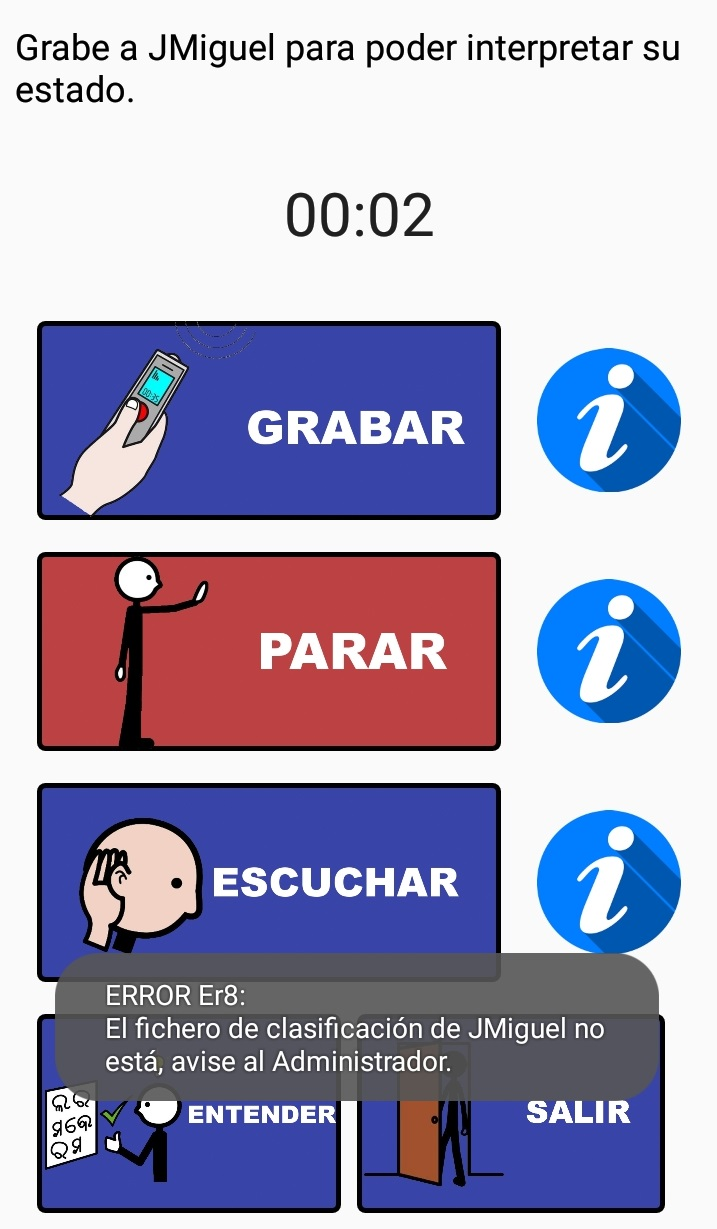
\includegraphics[scale=0.3]{error}
	\caption{Ejemplo de error.}
	\label{fig:error}
\end{figure}

Después de terminar de enlazar la aplicación de interpretación con el servidor, modifiqué y eliminé algunos test que tenía implementados, pudiendo así probar desde los test unitario y de integración el servidor. Al final, realicé un total de 82 test, como se puede ver en la figura~\ref{fig:test}, entre unitario y de integración, que prueban diferentes partes de la aplicación y el servidor.

\begin{figure}
	\centering
	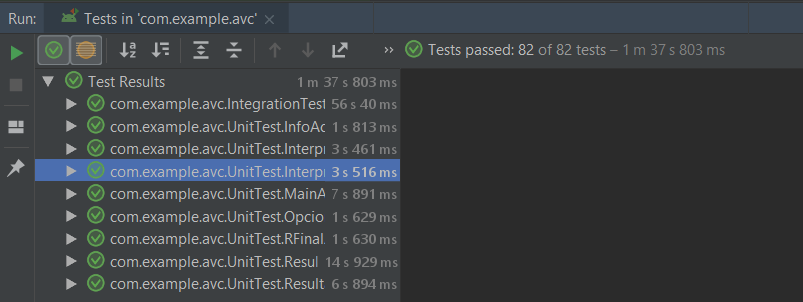
\includegraphics[width=\textwidth]{test}
	\caption{Resultado de los 82 test.}
	\label{fig:test}
\end{figure}

Con esto terminé el desarrollo de código del proyecto, pero no el proyecto en general ya que aún quedaba realizar presentaciones y documentarlo.

\section{Presentaciones y Premios}
Desde un principio nos pusimos como objetivo en el proyecto que éste fuese mediático, es decir, intentar apuntarnos al mayor número de presentaciones donde poder mostrar los avances del proyecto. A lo largo del desarrollo del proyecto he realizado, a diferentes tipos de públicos, las siguientes presentaciones:
\begin{itemize}
	\item Varias presentaciones en APACE de la aplicación de recogida de datos a los familiares y cuidadores del centro.
	\item Presentación de la aplicación final en las jornadas ASPACEnet en Madrid, 28 de Mayo de 2019. El certificado de asistencia se puede ver en la figura~\ref{fig:madrid}.
	\item Presentación para la elaboración del vídeo final del proyecto, \url{https://www.youtube.com/watch?v=6lWLMS9o8v0&feature=youtu.be}.
	\item Presentación de la aplicación final a los cuidadores del centro.
	\item Presentación ante la prensa del proyecto y de la aplicación~\ref{fig:presprensa}, la nota de prensa presencial se puede ver después de las líneas de trabajo futuras en el último apartado, y la nota de prensa digital se puede ver en  \url{https://www.diariodeburgos.es/Noticia/Z2D22B97F-0523-981F-1046FF5A06C5B81F/201906/Una-aplicacion-para-entender-a-quienes-no-pueden-hablar}.
\end{itemize}

\begin{figure}
	\centering
	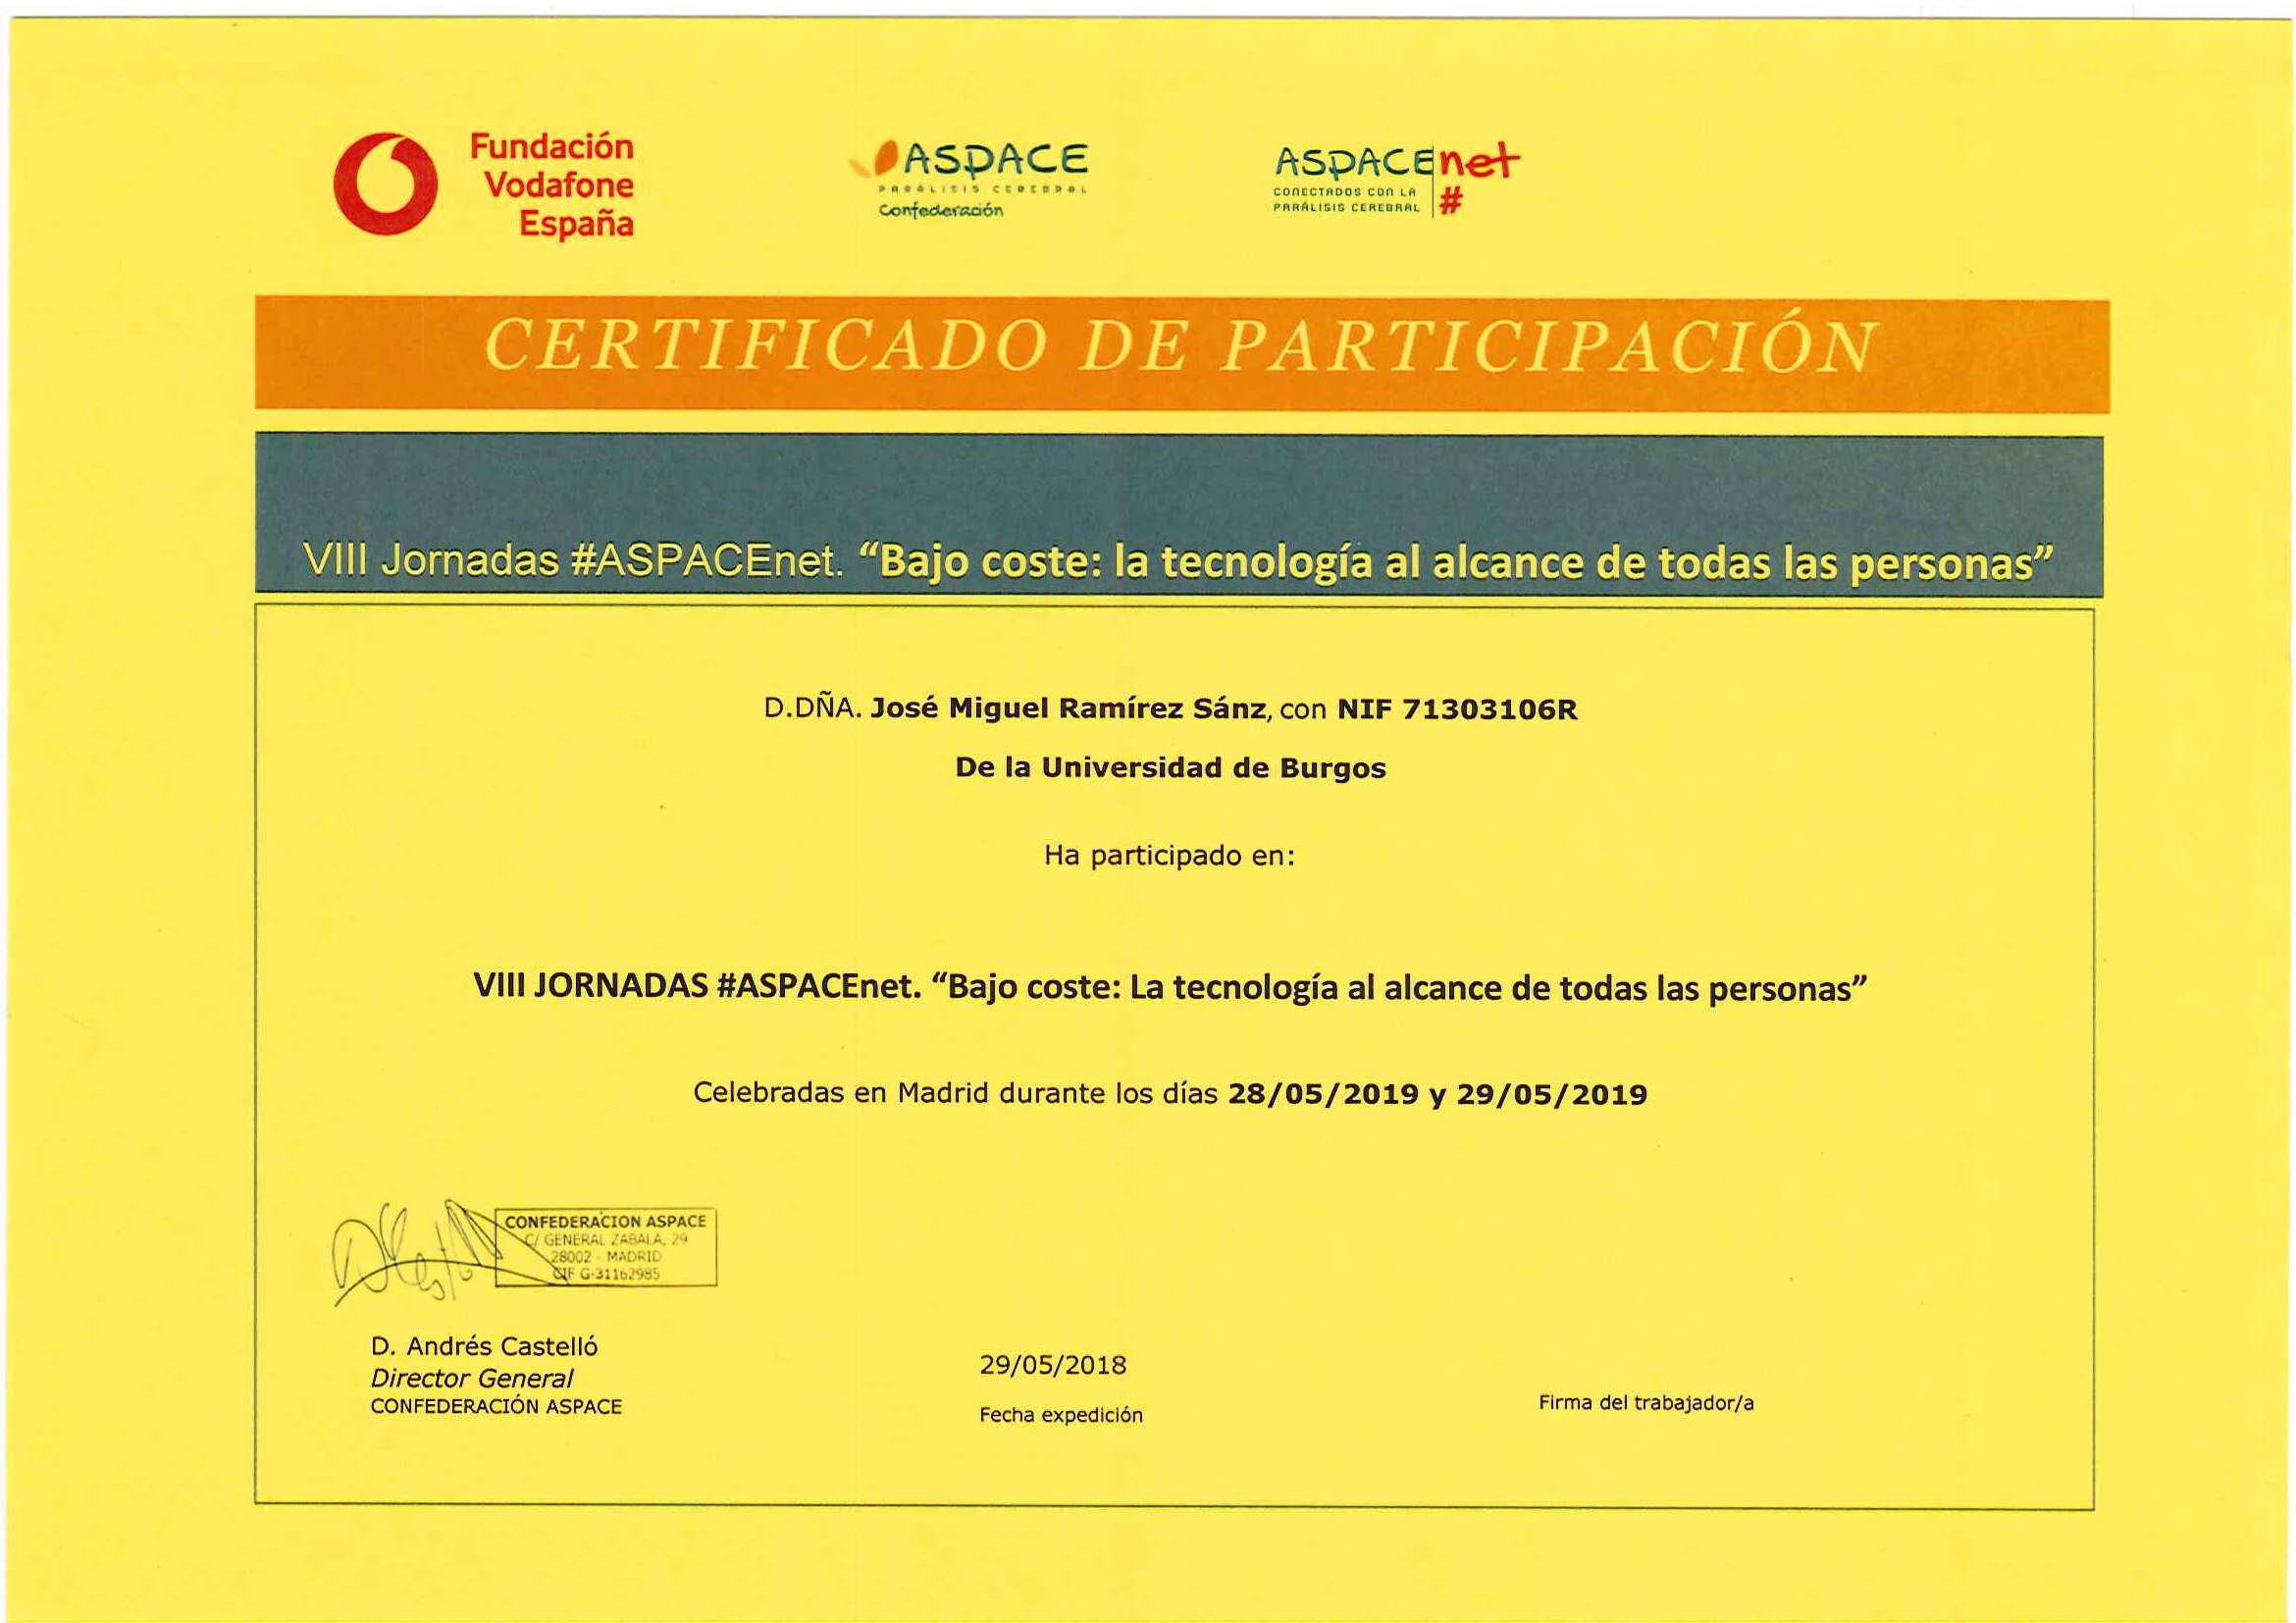
\includegraphics[width=\textwidth]{madrid}
	\caption{Certificado de asistencia a las jornadas ASPACEnet 2019 en Madrid.}
	\label{fig:madrid}
\end{figure}

\begin{figure}
	\centering
	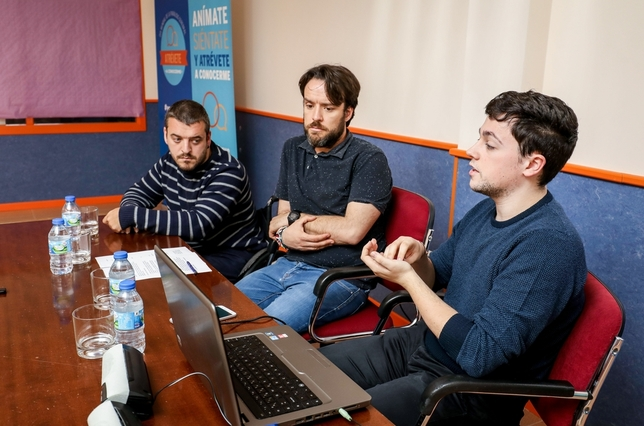
\includegraphics[width=\textwidth]{presentacionprensa}
	\caption{Imagen de la presentación ante la prensa, fuente \textit{Diario de Burgos}.}
	\label{fig:presprensa}
\end{figure}

El proyecto ha sido galardonado con los premios de Fundación Vodafone y de Becas Prototipo.